\documentclass[1p]{elsarticle_modified}
%\bibliographystyle{elsarticle-num}

%\usepackage[colorlinks]{hyperref}
%\usepackage{abbrmath_seonhwa} %\Abb, \Ascr, \Acal ,\Abf, \Afrak
\usepackage{amsfonts}
\usepackage{amssymb}
\usepackage{amsmath}
\usepackage{amsthm}
\usepackage{scalefnt}
\usepackage{amsbsy}
\usepackage{kotex}
\usepackage{caption}
\usepackage{subfig}
\usepackage{color}
\usepackage{graphicx}
\usepackage{xcolor} %% white, black, red, green, blue, cyan, magenta, yellow
\usepackage{float}
\usepackage{setspace}
\usepackage{hyperref}

\usepackage{tikz}
\usetikzlibrary{arrows}

\usepackage{multirow}
\usepackage{array} % fixed length table
\usepackage{hhline}

%%%%%%%%%%%%%%%%%%%%%
\makeatletter
\renewcommand*\env@matrix[1][\arraystretch]{%
	\edef\arraystretch{#1}%
	\hskip -\arraycolsep
	\let\@ifnextchar\new@ifnextchar
	\array{*\c@MaxMatrixCols c}}
\makeatother %https://tex.stackexchange.com/questions/14071/how-can-i-increase-the-line-spacing-in-a-matrix
%%%%%%%%%%%%%%%

\usepackage[normalem]{ulem}

\newcommand{\msout}[1]{\ifmmode\text{\sout{\ensuremath{#1}}}\else\sout{#1}\fi}
%SOURCE: \msout is \stkout macro in https://tex.stackexchange.com/questions/20609/strikeout-in-math-mode

\newcommand{\cancel}[1]{
	\ifmmode
	{\color{red}\msout{#1}}
	\else
	{\color{red}\sout{#1}}
	\fi
}

\newcommand{\add}[1]{
	{\color{blue}\uwave{#1}}
}

\newcommand{\replace}[2]{
	\ifmmode
	{\color{red}\msout{#1}}{\color{blue}\uwave{#2}}
	\else
	{\color{red}\sout{#1}}{\color{blue}\uwave{#2}}
	\fi
}

\newcommand{\Sol}{\mathcal{S}} %segment
\newcommand{\D}{D} %diagram
\newcommand{\A}{\mathcal{A}} %arc


%%%%%%%%%%%%%%%%%%%%%%%%%%%%%5 test

\def\sl{\operatorname{\textup{SL}}(2,\Cbb)}
\def\psl{\operatorname{\textup{PSL}}(2,\Cbb)}
\def\quan{\mkern 1mu \triangleright \mkern 1mu}

\theoremstyle{definition}
\newtheorem{thm}{Theorem}[section]
\newtheorem{prop}[thm]{Proposition}
\newtheorem{lem}[thm]{Lemma}
\newtheorem{ques}[thm]{Question}
\newtheorem{cor}[thm]{Corollary}
\newtheorem{defn}[thm]{Definition}
\newtheorem{exam}[thm]{Example}
\newtheorem{rmk}[thm]{Remark}
\newtheorem{alg}[thm]{Algorithm}

\newcommand{\I}{\sqrt{-1}}
\begin{document}

%\begin{frontmatter}
%
%\title{Boundary parabolic representations of knots up to 8 crossings}
%
%%% Group authors per affiliation:
%\author{Yunhi Cho} 
%\address{Department of Mathematics, University of Seoul, Seoul, Korea}
%\ead{yhcho@uos.ac.kr}
%
%
%\author{Seonhwa Kim} %\fnref{s_kim}}
%\address{Center for Geometry and Physics, Institute for Basic Science, Pohang, 37673, Korea}
%\ead{ryeona17@ibs.re.kr}
%
%\author{Hyuk Kim}
%\address{Department of Mathematical Sciences, Seoul National University, Seoul 08826, Korea}
%\ead{hyukkim@snu.ac.kr}
%
%\author{Seokbeom Yoon}
%\address{Department of Mathematical Sciences, Seoul National University, Seoul, 08826,  Korea}
%\ead{sbyoon15@snu.ac.kr}
%
%\begin{abstract}
%We find all boundary parabolic representation of knots up to 8 crossings.
%
%\end{abstract}
%\begin{keyword}
%    \MSC[2010] 57M25 
%\end{keyword}
%
%\end{frontmatter}

%\linenumbers
%\tableofcontents
%
\newcommand\colored[1]{\textcolor{white}{\rule[-0.35ex]{0.8em}{1.4ex}}\kern-0.8em\color{red} #1}%
%\newcommand\colored[1]{\textcolor{white}{ #1}\kern-2.17ex	\textcolor{white}{ #1}\kern-1.81ex	\textcolor{white}{ #1}\kern-2.15ex\color{red}#1	}

{\Large $\underline{11a_{269}~(K11a_{269})}$}

\setlength{\tabcolsep}{10pt}
\renewcommand{\arraystretch}{1.6}
\vspace{1cm}\begin{tabular}{m{100pt}>{\centering\arraybackslash}m{274pt}}
\multirow{5}{120pt}{
	\centering
	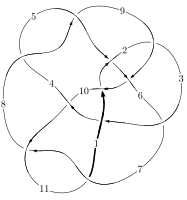
\includegraphics[width=112pt]{../../../GIT/diagram.site/Diagrams/png/518_11a_269.png}\\
\ \ \ A knot diagram\footnotemark}&
\allowdisplaybreaks
\textbf{Linearized knot diagam} \\
\cline{2-2}
 &
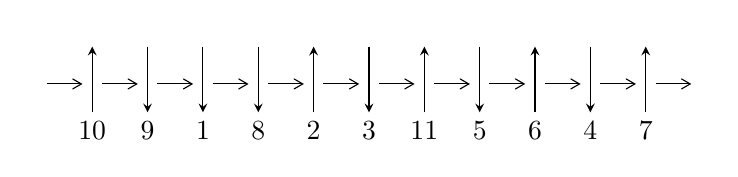
\begin{tikzpicture}[x=20pt, y=17pt]
	% nodes
	\node (C0) at (0, 0) {};
	\node (C1) at (1, 0) {};
	\node (C1U) at (1, +1) {};
	\node (C1D) at (1, -1) {10};

	\node (C2) at (2, 0) {};
	\node (C2U) at (2, +1) {};
	\node (C2D) at (2, -1) {9};

	\node (C3) at (3, 0) {};
	\node (C3U) at (3, +1) {};
	\node (C3D) at (3, -1) {1};

	\node (C4) at (4, 0) {};
	\node (C4U) at (4, +1) {};
	\node (C4D) at (4, -1) {8};

	\node (C5) at (5, 0) {};
	\node (C5U) at (5, +1) {};
	\node (C5D) at (5, -1) {2};

	\node (C6) at (6, 0) {};
	\node (C6U) at (6, +1) {};
	\node (C6D) at (6, -1) {3};

	\node (C7) at (7, 0) {};
	\node (C7U) at (7, +1) {};
	\node (C7D) at (7, -1) {11};

	\node (C8) at (8, 0) {};
	\node (C8U) at (8, +1) {};
	\node (C8D) at (8, -1) {5};

	\node (C9) at (9, 0) {};
	\node (C9U) at (9, +1) {};
	\node (C9D) at (9, -1) {6};

	\node (C10) at (10, 0) {};
	\node (C10U) at (10, +1) {};
	\node (C10D) at (10, -1) {4};

	\node (C11) at (11, 0) {};
	\node (C11U) at (11, +1) {};
	\node (C11D) at (11, -1) {7};
	\node (C12) at (12, 0) {};

	% arrows
	\draw[->,>={angle 60}]
	(C0) edge (C1) (C1) edge (C2) (C2) edge (C3) (C3) edge (C4) (C4) edge (C5) (C5) edge (C6) (C6) edge (C7) (C7) edge (C8) (C8) edge (C9) (C9) edge (C10) (C10) edge (C11) (C11) edge (C12) ;	\draw[->,>=stealth]
	(C1D) edge (C1U) (C2U) edge (C2D) (C3U) edge (C3D) (C4U) edge (C4D) (C5D) edge (C5U) (C6U) edge (C6D) (C7D) edge (C7U) (C8U) edge (C8D) (C9D) edge (C9U) (C10U) edge (C10D) (C11D) edge (C11U) ;
	\end{tikzpicture} \\
\hhline{~~} \\& 
\textbf{Solving Sequence} \\ \cline{2-2} 
 &
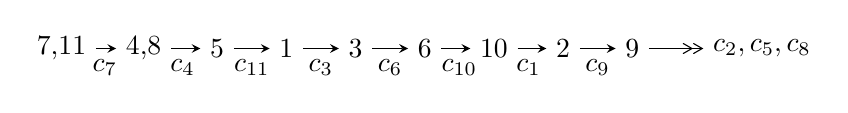
\begin{tikzpicture}[x=25pt, y=7pt]
	% node
	\node (A0) at (-1/8, 0) {7,11};
	\node (A1) at (17/16, 0) {4,8};
	\node (A2) at (17/8, 0) {5};
	\node (A3) at (25/8, 0) {1};
	\node (A4) at (33/8, 0) {3};
	\node (A5) at (41/8, 0) {6};
	\node (A6) at (49/8, 0) {10};
	\node (A7) at (57/8, 0) {2};
	\node (A8) at (65/8, 0) {9};
	\node (C1) at (1/2, -1) {$c_{7}$};
	\node (C2) at (13/8, -1) {$c_{4}$};
	\node (C3) at (21/8, -1) {$c_{11}$};
	\node (C4) at (29/8, -1) {$c_{3}$};
	\node (C5) at (37/8, -1) {$c_{6}$};
	\node (C6) at (45/8, -1) {$c_{10}$};
	\node (C7) at (53/8, -1) {$c_{1}$};
	\node (C8) at (61/8, -1) {$c_{9}$};
	\node (A9) at (10, 0) {$c_{2},c_{5},c_{8}$};

	% edge
	\draw[->,>=stealth]	
	(A0) edge (A1) (A1) edge (A2) (A2) edge (A3) (A3) edge (A4) (A4) edge (A5) (A5) edge (A6) (A6) edge (A7) (A7) edge (A8) ;
	\draw[->>,>={angle 60}]	
	(A8) edge (A9);
\end{tikzpicture} \\ 

\end{tabular} \\

\footnotetext{
The image of knot diagram is generated by the software ``\textbf{Draw programme}" developed by Andrew Bartholomew(\url{http://www.layer8.co.uk/maths/draw/index.htm\#Running-draw}), where we modified some parts for our purpose(\url{https://github.com/CATsTAILs/LinksPainter}).
}\phantom \\ \newline 
\centering \textbf{Ideals for irreducible components\footnotemark of $X_{\text{par}}$} 
 
\begin{align*}
I^u_{1}&=\langle 
-4.49185\times10^{277} u^{94}-2.89200\times10^{277} u^{93}+\cdots+3.55034\times10^{279} b+8.38424\times10^{277},\\
\phantom{I^u_{1}}&\phantom{= \langle  }9.85122\times10^{279} u^{94}+1.40469\times10^{279} u^{93}+\cdots+3.90538\times10^{280} a-1.47273\times10^{282},\\
\phantom{I^u_{1}}&\phantom{= \langle  }u^{95}+35 u^{93}+\cdots-304 u+31\rangle \\
I^u_{2}&=\langle 
-7910376 u^{19}+4613793 u^{18}+\cdots+11691787 b+11999209,\\
\phantom{I^u_{2}}&\phantom{= \langle  }5476396 u^{19}-5762435 u^{18}+\cdots+11691787 a-44515827,\;u^{20}- u^{19}+\cdots-4 u-1\rangle \\
\\
\end{align*}
\raggedright * 2 irreducible components of $\dim_{\mathbb{C}}=0$, with total 115 representations.\\
\footnotetext{All coefficients of polynomials are rational numbers. But the coefficients are sometimes approximated in decimal forms when there is not enough margin.}
\newpage
\renewcommand{\arraystretch}{1}
\centering \section*{I. $I^u_{1}= \langle -4.49\times10^{277} u^{94}-2.89\times10^{277} u^{93}+\cdots+3.55\times10^{279} b+8.38\times10^{277},\;9.85\times10^{279} u^{94}+1.40\times10^{279} u^{93}+\cdots+3.91\times10^{280} a-1.47\times10^{282},\;u^{95}+35 u^{93}+\cdots-304 u+31 \rangle$}
\flushleft \textbf{(i) Arc colorings}\\
\begin{tabular}{m{7pt} m{180pt} m{7pt} m{180pt} }
\flushright $a_{7}=$&$\begin{pmatrix}1\\0\end{pmatrix}$ \\
\flushright $a_{11}=$&$\begin{pmatrix}0\\u\end{pmatrix}$ \\
\flushright $a_{4}=$&$\begin{pmatrix}-0.252248 u^{94}-0.0359681 u^{93}+\cdots-187.834 u+37.7103\\0.0126519 u^{94}+0.00814570 u^{93}+\cdots+6.14641 u-0.0236153\end{pmatrix}$ \\
\flushright $a_{8}=$&$\begin{pmatrix}1\\- u^2\end{pmatrix}$ \\
\flushright $a_{5}=$&$\begin{pmatrix}-0.223306 u^{94}+0.0151371 u^{93}+\cdots-190.866 u+36.6189\\0.0215402 u^{94}+0.0658023 u^{93}+\cdots-8.49240 u+1.56065\end{pmatrix}$ \\
\flushright $a_{1}=$&$\begin{pmatrix}u\\u\end{pmatrix}$ \\
\flushright $a_{3}=$&$\begin{pmatrix}-0.228927 u^{94}-0.00653034 u^{93}+\cdots-182.635 u+36.3428\\0.0359728 u^{94}+0.0375835 u^{93}+\cdots+11.3451 u-1.39114\end{pmatrix}$ \\
\flushright $a_{6}=$&$\begin{pmatrix}0.132211 u^{94}+0.0353042 u^{93}+\cdots+52.2661 u-13.3444\\-0.0286481 u^{94}-0.0274990 u^{93}+\cdots-27.6589 u+3.67427\end{pmatrix}$ \\
\flushright $a_{10}=$&$\begin{pmatrix}-0.588967 u^{94}-0.122495 u^{93}+\cdots-451.158 u+79.6285\\-0.0215088 u^{94}+0.00726948 u^{93}+\cdots-43.9334 u+8.03715\end{pmatrix}$ \\
\flushright $a_{2}=$&$\begin{pmatrix}-1.04919 u^{94}-0.197484 u^{93}+\cdots-719.135 u+125.759\\-0.278898 u^{94}-0.00407899 u^{93}+\cdots-166.161 u+28.6179\end{pmatrix}$ \\
\flushright $a_{9}=$&$\begin{pmatrix}-0.332719 u^{94}-0.0981982 u^{93}+\cdots-254.739 u+49.5570\\0.0297838 u^{94}+0.00801573 u^{93}+\cdots+7.57210 u+0.539403\end{pmatrix}$\\ \flushright $a_{9}=$&$\begin{pmatrix}-0.332719 u^{94}-0.0981982 u^{93}+\cdots-254.739 u+49.5570\\0.0297838 u^{94}+0.00801573 u^{93}+\cdots+7.57210 u+0.539403\end{pmatrix}$\\&\end{tabular}
\flushleft \textbf{(ii) Obstruction class $= -1$}\\~\\
\flushleft \textbf{(iii) Cusp Shapes $= -0.425242 u^{94}-0.172495 u^{93}+\cdots-151.920 u+18.7514$}\\~\\
\newpage\renewcommand{\arraystretch}{1}
\flushleft \textbf{(iv) u-Polynomials at the component}\newline \\
\begin{tabular}{m{50pt}|m{274pt}}
Crossings & \hspace{64pt}u-Polynomials at each crossing \\
\hline $$\begin{aligned}c_{1}\end{aligned}$$&$\begin{aligned}
&u^{95}+8 u^{94}+\cdots-1011270 u-170729
\end{aligned}$\\
\hline $$\begin{aligned}c_{2}\end{aligned}$$&$\begin{aligned}
&u^{95}+3 u^{94}+\cdots+6615 u-451
\end{aligned}$\\
\hline $$\begin{aligned}c_{3}\end{aligned}$$&$\begin{aligned}
&u^{95}+6 u^{94}+\cdots+2006 u+1867
\end{aligned}$\\
\hline $$\begin{aligned}c_{4},c_{8}\end{aligned}$$&$\begin{aligned}
&u^{95}+5 u^{94}+\cdots+290 u+31
\end{aligned}$\\
\hline $$\begin{aligned}c_{5}\end{aligned}$$&$\begin{aligned}
&u^{95}- u^{94}+\cdots-4620 u-413
\end{aligned}$\\
\hline $$\begin{aligned}c_{6}\end{aligned}$$&$\begin{aligned}
&u^{95}-2 u^{94}+\cdots-4406294 u-7707151
\end{aligned}$\\
\hline $$\begin{aligned}c_{7},c_{11}\end{aligned}$$&$\begin{aligned}
&u^{95}+35 u^{93}+\cdots-304 u-31
\end{aligned}$\\
\hline $$\begin{aligned}c_{9}\end{aligned}$$&$\begin{aligned}
&u^{95}+u^{94}+\cdots-13 u-1
\end{aligned}$\\
\hline $$\begin{aligned}c_{10}\end{aligned}$$&$\begin{aligned}
&u^{95}-23 u^{93}+\cdots-51128 u+2537
\end{aligned}$\\
\hline
\end{tabular}\\~\\
\newpage\renewcommand{\arraystretch}{1}
\flushleft \textbf{(v) Riley Polynomials at the component}\newline \\
\begin{tabular}{m{50pt}|m{274pt}}
Crossings & \hspace{64pt}Riley Polynomials at each crossing \\
\hline $$\begin{aligned}c_{1}\end{aligned}$$&$\begin{aligned}
&y^{95}+32 y^{94}+\cdots-975808808676 y-29148391441
\end{aligned}$\\
\hline $$\begin{aligned}c_{2}\end{aligned}$$&$\begin{aligned}
&y^{95}-33 y^{94}+\cdots+5314083 y-203401
\end{aligned}$\\
\hline $$\begin{aligned}c_{3}\end{aligned}$$&$\begin{aligned}
&y^{95}-34 y^{94}+\cdots+99285844 y-3485689
\end{aligned}$\\
\hline $$\begin{aligned}c_{4},c_{8}\end{aligned}$$&$\begin{aligned}
&y^{95}-89 y^{94}+\cdots-142386 y-961
\end{aligned}$\\
\hline $$\begin{aligned}c_{5}\end{aligned}$$&$\begin{aligned}
&y^{95}+23 y^{94}+\cdots-4607694 y-170569
\end{aligned}$\\
\hline $$\begin{aligned}c_{6}\end{aligned}$$&$\begin{aligned}
&y^{95}-58 y^{94}+\cdots+1536043799096208 y-59400176536801
\end{aligned}$\\
\hline $$\begin{aligned}c_{7},c_{11}\end{aligned}$$&$\begin{aligned}
&y^{95}+70 y^{94}+\cdots+1958 y-961
\end{aligned}$\\
\hline $$\begin{aligned}c_{9}\end{aligned}$$&$\begin{aligned}
&y^{95}+11 y^{94}+\cdots-61 y-1
\end{aligned}$\\
\hline $$\begin{aligned}c_{10}\end{aligned}$$&$\begin{aligned}
&y^{95}-46 y^{94}+\cdots+1721708004 y-6436369
\end{aligned}$\\
\hline
\end{tabular}\\~\\
\newpage\flushleft \textbf{(vi) Complex Volumes and Cusp Shapes}
$$\begin{array}{c|c|c}  
\text{Solutions to }I^u_{1}& \I (\text{vol} + \sqrt{-1}CS) & \text{Cusp shape}\\
 \hline 
\begin{aligned}
u &= \phantom{-}0.203044 + 0.917129 I \\
a &= -0.072460 + 0.599163 I \\
b &= -1.83757 + 1.44426 I\end{aligned}
 & -4.56432 + 0.25339 I & \phantom{-0.000000 } 0 \\ \hline\begin{aligned}
u &= \phantom{-}0.203044 - 0.917129 I \\
a &= -0.072460 - 0.599163 I \\
b &= -1.83757 - 1.44426 I\end{aligned}
 & -4.56432 - 0.25339 I & \phantom{-0.000000 } 0 \\ \hline\begin{aligned}
u &= \phantom{-}0.188818 + 1.046850 I \\
a &= \phantom{-}0.353704 + 1.363350 I \\
b &= \phantom{-}0.82428 + 2.06012 I\end{aligned}
 & -1.00596 + 4.93534 I & \phantom{-0.000000 } 0 \\ \hline\begin{aligned}
u &= \phantom{-}0.188818 - 1.046850 I \\
a &= \phantom{-}0.353704 - 1.363350 I \\
b &= \phantom{-}0.82428 - 2.06012 I\end{aligned}
 & -1.00596 - 4.93534 I & \phantom{-0.000000 } 0 \\ \hline\begin{aligned}
u &= -0.841903 + 0.379537 I \\
a &= -1.46081 - 0.05491 I \\
b &= -0.451611 - 0.818600 I\end{aligned}
 & -3.29557 + 3.88851 I & \phantom{-0.000000 } 0 \\ \hline\begin{aligned}
u &= -0.841903 - 0.379537 I \\
a &= -1.46081 + 0.05491 I \\
b &= -0.451611 + 0.818600 I\end{aligned}
 & -3.29557 - 3.88851 I & \phantom{-0.000000 } 0 \\ \hline\begin{aligned}
u &= \phantom{-}0.174169 + 0.902857 I \\
a &= \phantom{-}0.014969 - 0.537441 I \\
b &= -0.646019 - 1.176240 I\end{aligned}
 & \phantom{-}0.131344 - 1.193480 I & \phantom{-0.000000 } 0 \\ \hline\begin{aligned}
u &= \phantom{-}0.174169 - 0.902857 I \\
a &= \phantom{-}0.014969 + 0.537441 I \\
b &= -0.646019 + 1.176240 I\end{aligned}
 & \phantom{-}0.131344 + 1.193480 I & \phantom{-0.000000 } 0 \\ \hline\begin{aligned}
u &= \phantom{-}0.781278 + 0.449701 I \\
a &= \phantom{-}0.482897 - 1.147300 I \\
b &= \phantom{-}0.258543 + 0.080747 I\end{aligned}
 & -3.83969 + 3.68020 I & \phantom{-0.000000 } 0 \\ \hline\begin{aligned}
u &= \phantom{-}0.781278 - 0.449701 I \\
a &= \phantom{-}0.482897 + 1.147300 I \\
b &= \phantom{-}0.258543 - 0.080747 I\end{aligned}
 & -3.83969 - 3.68020 I & \phantom{-0.000000 } 0\\
 \hline 
 \end{array}$$\newpage$$\begin{array}{c|c|c}  
\text{Solutions to }I^u_{1}& \I (\text{vol} + \sqrt{-1}CS) & \text{Cusp shape}\\
 \hline 
\begin{aligned}
u &= \phantom{-}0.147761 + 1.110270 I \\
a &= -0.464772 + 0.570801 I \\
b &= -0.45030 + 1.94664 I\end{aligned}
 & -4.51152 + 0.64108 I & \phantom{-0.000000 } 0 \\ \hline\begin{aligned}
u &= \phantom{-}0.147761 - 1.110270 I \\
a &= -0.464772 - 0.570801 I \\
b &= -0.45030 - 1.94664 I\end{aligned}
 & -4.51152 - 0.64108 I & \phantom{-0.000000 } 0 \\ \hline\begin{aligned}
u &= \phantom{-}0.873588 + 0.053551 I \\
a &= -0.864438 - 0.922058 I \\
b &= \phantom{-}0.277114 - 0.192656 I\end{aligned}
 & -0.90223 - 7.26936 I & \phantom{-0.000000 -}0. + 7.70751 I \\ \hline\begin{aligned}
u &= \phantom{-}0.873588 - 0.053551 I \\
a &= -0.864438 + 0.922058 I \\
b &= \phantom{-}0.277114 + 0.192656 I\end{aligned}
 & -0.90223 + 7.26936 I & \phantom{-0.000000 } 0. - 7.70751 I \\ \hline\begin{aligned}
u &= -0.853098 + 0.138319 I \\
a &= \phantom{-}0.467239 - 0.646604 I \\
b &= \phantom{-}0.227419 + 0.058231 I\end{aligned}
 & \phantom{-}2.42910 - 0.66447 I & \phantom{-0.000000 } 0 \\ \hline\begin{aligned}
u &= -0.853098 - 0.138319 I \\
a &= \phantom{-}0.467239 + 0.646604 I \\
b &= \phantom{-}0.227419 - 0.058231 I\end{aligned}
 & \phantom{-}2.42910 + 0.66447 I & \phantom{-0.000000 } 0 \\ \hline\begin{aligned}
u &= -0.214908 + 1.153540 I \\
a &= \phantom{-}0.207367 - 0.595525 I \\
b &= \phantom{-}0.49768 - 2.75342 I\end{aligned}
 & -4.42358 - 0.93929 I & \phantom{-0.000000 } 0 \\ \hline\begin{aligned}
u &= -0.214908 - 1.153540 I \\
a &= \phantom{-}0.207367 + 0.595525 I \\
b &= \phantom{-}0.49768 + 2.75342 I\end{aligned}
 & -4.42358 + 0.93929 I & \phantom{-0.000000 } 0 \\ \hline\begin{aligned}
u &= -0.410035 + 1.106710 I \\
a &= \phantom{-}0.19753 + 1.95483 I \\
b &= -0.21279 + 2.51734 I\end{aligned}
 & -5.58860 - 8.53903 I & \phantom{-0.000000 } 0 \\ \hline\begin{aligned}
u &= -0.410035 - 1.106710 I \\
a &= \phantom{-}0.19753 - 1.95483 I \\
b &= -0.21279 - 2.51734 I\end{aligned}
 & -5.58860 + 8.53903 I & \phantom{-0.000000 } 0\\
 \hline 
 \end{array}$$\newpage$$\begin{array}{c|c|c}  
\text{Solutions to }I^u_{1}& \I (\text{vol} + \sqrt{-1}CS) & \text{Cusp shape}\\
 \hline 
\begin{aligned}
u &= \phantom{-}0.065053 + 1.185530 I \\
a &= -1.088310 + 0.080842 I \\
b &= -0.004477 + 0.558757 I\end{aligned}
 & -5.52730 + 1.54119 I & \phantom{-0.000000 } 0 \\ \hline\begin{aligned}
u &= \phantom{-}0.065053 - 1.185530 I \\
a &= -1.088310 - 0.080842 I \\
b &= -0.004477 - 0.558757 I\end{aligned}
 & -5.52730 - 1.54119 I & \phantom{-0.000000 } 0 \\ \hline\begin{aligned}
u &= \phantom{-}1.182220 + 0.171664 I \\
a &= -0.825483 + 0.487836 I \\
b &= -0.135537 + 0.091551 I\end{aligned}
 & -6.11822 + 3.45479 I & \phantom{-0.000000 } 0 \\ \hline\begin{aligned}
u &= \phantom{-}1.182220 - 0.171664 I \\
a &= -0.825483 - 0.487836 I \\
b &= -0.135537 - 0.091551 I\end{aligned}
 & -6.11822 - 3.45479 I & \phantom{-0.000000 } 0 \\ \hline\begin{aligned}
u &= \phantom{-}0.015472 + 1.211050 I \\
a &= \phantom{-}2.13863 - 1.20659 I \\
b &= \phantom{-}1.76210 - 1.71409 I\end{aligned}
 & -8.90213 + 6.92952 I & \phantom{-0.000000 } 0 \\ \hline\begin{aligned}
u &= \phantom{-}0.015472 - 1.211050 I \\
a &= \phantom{-}2.13863 + 1.20659 I \\
b &= \phantom{-}1.76210 + 1.71409 I\end{aligned}
 & -8.90213 - 6.92952 I & \phantom{-0.000000 } 0 \\ \hline\begin{aligned}
u &= -0.300875 + 1.186360 I \\
a &= -1.056320 - 0.895869 I \\
b &= -0.87032 - 1.56886 I\end{aligned}
 & -4.85814 - 5.15679 I & \phantom{-0.000000 } 0 \\ \hline\begin{aligned}
u &= -0.300875 - 1.186360 I \\
a &= -1.056320 + 0.895869 I \\
b &= -0.87032 + 1.56886 I\end{aligned}
 & -4.85814 + 5.15679 I & \phantom{-0.000000 } 0 \\ \hline\begin{aligned}
u &= -0.597468 + 0.471809 I \\
a &= \phantom{-}0.387239 - 1.071350 I \\
b &= \phantom{-}0.447471 - 0.089097 I\end{aligned}
 & \phantom{-}0.16031 - 2.08239 I & \phantom{-}3.28409 + 5.43220 I \\ \hline\begin{aligned}
u &= -0.597468 - 0.471809 I \\
a &= \phantom{-}0.387239 + 1.071350 I \\
b &= \phantom{-}0.447471 + 0.089097 I\end{aligned}
 & \phantom{-}0.16031 + 2.08239 I & \phantom{-}3.28409 - 5.43220 I\\
 \hline 
 \end{array}$$\newpage$$\begin{array}{c|c|c}  
\text{Solutions to }I^u_{1}& \I (\text{vol} + \sqrt{-1}CS) & \text{Cusp shape}\\
 \hline 
\begin{aligned}
u &= \phantom{-}0.373977 + 1.191530 I \\
a &= -0.508278 - 1.136990 I \\
b &= -0.234912 - 1.231560 I\end{aligned}
 & -5.82363 + 4.27424 I & \phantom{-0.000000 } 0 \\ \hline\begin{aligned}
u &= \phantom{-}0.373977 - 1.191530 I \\
a &= -0.508278 + 1.136990 I \\
b &= -0.234912 + 1.231560 I\end{aligned}
 & -5.82363 - 4.27424 I & \phantom{-0.000000 } 0 \\ \hline\begin{aligned}
u &= \phantom{-}0.126110 + 1.254030 I \\
a &= \phantom{-}1.06317 + 1.57024 I \\
b &= \phantom{-}0.78981 + 2.36764 I\end{aligned}
 & -9.12386 + 3.30593 I & \phantom{-0.000000 } 0 \\ \hline\begin{aligned}
u &= \phantom{-}0.126110 - 1.254030 I \\
a &= \phantom{-}1.06317 - 1.57024 I \\
b &= \phantom{-}0.78981 - 2.36764 I\end{aligned}
 & -9.12386 - 3.30593 I & \phantom{-0.000000 } 0 \\ \hline\begin{aligned}
u &= -1.253650 + 0.190827 I \\
a &= \phantom{-}0.743113 + 0.527927 I \\
b &= \phantom{-}0.0522154 - 0.1040810 I\end{aligned}
 & -6.46116 - 11.90460 I & \phantom{-0.000000 } 0 \\ \hline\begin{aligned}
u &= -1.253650 - 0.190827 I \\
a &= \phantom{-}0.743113 - 0.527927 I \\
b &= \phantom{-}0.0522154 + 0.1040810 I\end{aligned}
 & -6.46116 + 11.90460 I & \phantom{-0.000000 } 0 \\ \hline\begin{aligned}
u &= \phantom{-}0.015327 + 1.271330 I \\
a &= \phantom{-}0.422614 + 1.071250 I \\
b &= -0.64580 + 2.04830 I\end{aligned}
 & -9.14776 - 1.14213 I & \phantom{-0.000000 } 0 \\ \hline\begin{aligned}
u &= \phantom{-}0.015327 - 1.271330 I \\
a &= \phantom{-}0.422614 - 1.071250 I \\
b &= -0.64580 - 2.04830 I\end{aligned}
 & -9.14776 + 1.14213 I & \phantom{-0.000000 } 0 \\ \hline\begin{aligned}
u &= -0.377285 + 1.214920 I \\
a &= \phantom{-}0.289098 - 0.998400 I \\
b &= \phantom{-}0.47140 - 1.69716 I\end{aligned}
 & -0.92977 - 3.70164 I & \phantom{-0.000000 } 0 \\ \hline\begin{aligned}
u &= -0.377285 - 1.214920 I \\
a &= \phantom{-}0.289098 + 0.998400 I \\
b &= \phantom{-}0.47140 + 1.69716 I\end{aligned}
 & -0.92977 + 3.70164 I & \phantom{-0.000000 } 0\\
 \hline 
 \end{array}$$\newpage$$\begin{array}{c|c|c}  
\text{Solutions to }I^u_{1}& \I (\text{vol} + \sqrt{-1}CS) & \text{Cusp shape}\\
 \hline 
\begin{aligned}
u &= -1.288570 + 0.007471 I \\
a &= -0.818723 - 0.198916 I \\
b &= \phantom{-}0.042763 + 0.289683 I\end{aligned}
 & -5.36768 - 2.13610 I & \phantom{-0.000000 } 0 \\ \hline\begin{aligned}
u &= -1.288570 - 0.007471 I \\
a &= -0.818723 + 0.198916 I \\
b &= \phantom{-}0.042763 - 0.289683 I\end{aligned}
 & -5.36768 + 2.13610 I & \phantom{-0.000000 } 0 \\ \hline\begin{aligned}
u &= \phantom{-}0.096861 + 1.285190 I \\
a &= -1.29489 - 1.50125 I \\
b &= -1.21097 - 2.02058 I\end{aligned}
 & -9.26018 + 1.58608 I & \phantom{-0.000000 } 0 \\ \hline\begin{aligned}
u &= \phantom{-}0.096861 - 1.285190 I \\
a &= -1.29489 + 1.50125 I \\
b &= -1.21097 + 2.02058 I\end{aligned}
 & -9.26018 - 1.58608 I & \phantom{-0.000000 } 0 \\ \hline\begin{aligned}
u &= \phantom{-}0.318977 + 1.271910 I \\
a &= -0.049631 + 0.924265 I \\
b &= \phantom{-}0.55142 + 2.17316 I\end{aligned}
 & -5.15661 + 5.20956 I & \phantom{-0.000000 } 0 \\ \hline\begin{aligned}
u &= \phantom{-}0.318977 - 1.271910 I \\
a &= -0.049631 - 0.924265 I \\
b &= \phantom{-}0.55142 - 2.17316 I\end{aligned}
 & -5.15661 - 5.20956 I & \phantom{-0.000000 } 0 \\ \hline\begin{aligned}
u &= \phantom{-}0.475645 + 0.496446 I \\
a &= -1.02531 - 1.03413 I \\
b &= \phantom{-}0.272472 + 0.084254 I\end{aligned}
 & \phantom{-}1.39130 + 4.10735 I & \phantom{-}0.47882 - 9.23280 I \\ \hline\begin{aligned}
u &= \phantom{-}0.475645 - 0.496446 I \\
a &= -1.02531 + 1.03413 I \\
b &= \phantom{-}0.272472 - 0.084254 I\end{aligned}
 & \phantom{-}1.39130 - 4.10735 I & \phantom{-}0.47882 + 9.23280 I \\ \hline\begin{aligned}
u &= -0.092319 + 1.316330 I \\
a &= \phantom{-}0.312500 - 0.740469 I \\
b &= -1.02183 - 1.77722 I\end{aligned}
 & -10.61240 - 8.00084 I & \phantom{-0.000000 } 0 \\ \hline\begin{aligned}
u &= -0.092319 - 1.316330 I \\
a &= \phantom{-}0.312500 + 0.740469 I \\
b &= -1.02183 + 1.77722 I\end{aligned}
 & -10.61240 + 8.00084 I & \phantom{-0.000000 } 0\\
 \hline 
 \end{array}$$\newpage$$\begin{array}{c|c|c}  
\text{Solutions to }I^u_{1}& \I (\text{vol} + \sqrt{-1}CS) & \text{Cusp shape}\\
 \hline 
\begin{aligned}
u &= \phantom{-}0.403900 + 1.270130 I \\
a &= -0.297287 - 0.873496 I \\
b &= -0.68395 - 2.26832 I\end{aligned}
 & -4.71304 + 11.85200 I & \phantom{-0.000000 } 0 \\ \hline\begin{aligned}
u &= \phantom{-}0.403900 - 1.270130 I \\
a &= -0.297287 + 0.873496 I \\
b &= -0.68395 + 2.26832 I\end{aligned}
 & -4.71304 - 11.85200 I & \phantom{-0.000000 } 0 \\ \hline\begin{aligned}
u &= \phantom{-}0.646591\phantom{ +0.000000I} \\
a &= -0.343975\phantom{ +0.000000I} \\
b &= -1.02884\phantom{ +0.000000I}\end{aligned}
 & -2.63135\phantom{ +0.000000I} & -2.77190\phantom{ +0.000000I} \\ \hline\begin{aligned}
u &= -0.190459 + 0.613907 I \\
a &= \phantom{-}0.478623 - 0.574775 I \\
b &= -0.017788 - 0.619736 I\end{aligned}
 & -0.082881 - 1.263940 I & -0.49456 + 4.76991 I \\ \hline\begin{aligned}
u &= -0.190459 - 0.613907 I \\
a &= \phantom{-}0.478623 + 0.574775 I \\
b &= -0.017788 + 0.619736 I\end{aligned}
 & -0.082881 + 1.263940 I & -0.49456 - 4.76991 I \\ \hline\begin{aligned}
u &= -0.218133 + 1.353350 I \\
a &= -0.248608 + 0.800951 I \\
b &= -0.86184 + 1.96783 I\end{aligned}
 & -5.40102 - 4.78928 I & \phantom{-0.000000 } 0 \\ \hline\begin{aligned}
u &= -0.218133 - 1.353350 I \\
a &= -0.248608 - 0.800951 I \\
b &= -0.86184 - 1.96783 I\end{aligned}
 & -5.40102 + 4.78928 I & \phantom{-0.000000 } 0 \\ \hline\begin{aligned}
u &= \phantom{-}0.559623 + 0.272141 I \\
a &= -0.294821 - 0.389565 I \\
b &= -1.142410 + 0.129341 I\end{aligned}
 & -2.66399 - 0.03648 I & -5.52133 - 0.36616 I \\ \hline\begin{aligned}
u &= \phantom{-}0.559623 - 0.272141 I \\
a &= -0.294821 + 0.389565 I \\
b &= -1.142410 - 0.129341 I\end{aligned}
 & -2.66399 + 0.03648 I & -5.52133 + 0.36616 I \\ \hline\begin{aligned}
u &= \phantom{-}0.282479 + 1.349510 I \\
a &= \phantom{-}0.555402 - 0.636749 I \\
b &= \phantom{-}0.606958 - 1.255200 I\end{aligned}
 & -5.51333 - 3.00258 I & \phantom{-0.000000 } 0\\
 \hline 
 \end{array}$$\newpage$$\begin{array}{c|c|c}  
\text{Solutions to }I^u_{1}& \I (\text{vol} + \sqrt{-1}CS) & \text{Cusp shape}\\
 \hline 
\begin{aligned}
u &= \phantom{-}0.282479 - 1.349510 I \\
a &= \phantom{-}0.555402 + 0.636749 I \\
b &= \phantom{-}0.606958 + 1.255200 I\end{aligned}
 & -5.51333 + 3.00258 I & \phantom{-0.000000 } 0 \\ \hline\begin{aligned}
u &= \phantom{-}0.605423 + 0.041300 I \\
a &= \phantom{-}1.069190 + 0.701968 I \\
b &= -0.402539 - 0.202573 I\end{aligned}
 & -1.33339 - 1.63852 I & -3.10982 + 5.30448 I \\ \hline\begin{aligned}
u &= \phantom{-}0.605423 - 0.041300 I \\
a &= \phantom{-}1.069190 - 0.701968 I \\
b &= -0.402539 + 0.202573 I\end{aligned}
 & -1.33339 + 1.63852 I & -3.10982 - 5.30448 I \\ \hline\begin{aligned}
u &= -0.453504 + 1.318710 I \\
a &= -0.051826 + 0.472508 I \\
b &= -0.451784 + 1.214970 I\end{aligned}
 & -2.17172 - 5.56944 I & \phantom{-0.000000 } 0 \\ \hline\begin{aligned}
u &= -0.453504 - 1.318710 I \\
a &= -0.051826 - 0.472508 I \\
b &= -0.451784 - 1.214970 I\end{aligned}
 & -2.17172 + 5.56944 I & \phantom{-0.000000 } 0 \\ \hline\begin{aligned}
u &= -1.40514\phantom{ +0.000000I} \\
a &= \phantom{-}0.0463063\phantom{ +0.000000I} \\
b &= \phantom{-}0.207522\phantom{ +0.000000I}\end{aligned}
 & \phantom{-}2.64340\phantom{ +0.000000I} & \phantom{-0.000000 } 0 \\ \hline\begin{aligned}
u &= -0.10693 + 1.42071 I \\
a &= -0.217725 + 0.645099 I \\
b &= \phantom{-}0.78436 + 1.54264 I\end{aligned}
 & -9.79145 + 0.88028 I & \phantom{-0.000000 } 0 \\ \hline\begin{aligned}
u &= -0.10693 - 1.42071 I \\
a &= -0.217725 - 0.645099 I \\
b &= \phantom{-}0.78436 - 1.54264 I\end{aligned}
 & -9.79145 - 0.88028 I & \phantom{-0.000000 } 0 \\ \hline\begin{aligned}
u &= -0.566959 + 0.058673 I \\
a &= \phantom{-}1.31839 - 1.05059 I \\
b &= -0.369297 - 0.610238 I\end{aligned}
 & -1.32796 - 2.03593 I & -2.81091 + 4.02942 I \\ \hline\begin{aligned}
u &= -0.566959 - 0.058673 I \\
a &= \phantom{-}1.31839 + 1.05059 I \\
b &= -0.369297 + 0.610238 I\end{aligned}
 & -1.32796 + 2.03593 I & -2.81091 - 4.02942 I\\
 \hline 
 \end{array}$$\newpage$$\begin{array}{c|c|c}  
\text{Solutions to }I^u_{1}& \I (\text{vol} + \sqrt{-1}CS) & \text{Cusp shape}\\
 \hline 
\begin{aligned}
u &= \phantom{-}0.240869 + 0.488806 I \\
a &= \phantom{-}2.31131 - 0.20191 I \\
b &= \phantom{-}0.279330 - 0.414621 I\end{aligned}
 & \phantom{-}0.77353 - 2.77220 I & \phantom{-}4.28354 - 5.94685 I \\ \hline\begin{aligned}
u &= \phantom{-}0.240869 - 0.488806 I \\
a &= \phantom{-}2.31131 + 0.20191 I \\
b &= \phantom{-}0.279330 + 0.414621 I\end{aligned}
 & \phantom{-}0.77353 + 2.77220 I & \phantom{-}4.28354 + 5.94685 I \\ \hline\begin{aligned}
u &= \phantom{-}0.268380 + 0.438809 I \\
a &= \phantom{-}0.07544 + 1.52989 I \\
b &= -1.41741 - 0.11606 I\end{aligned}
 & -4.35844 + 0.30967 I & -6.81908 + 1.81849 I \\ \hline\begin{aligned}
u &= \phantom{-}0.268380 - 0.438809 I \\
a &= \phantom{-}0.07544 - 1.52989 I \\
b &= -1.41741 + 0.11606 I\end{aligned}
 & -4.35844 - 0.30967 I & -6.81908 - 1.81849 I \\ \hline\begin{aligned}
u &= \phantom{-}0.48430 + 1.43457 I \\
a &= -0.316264 - 1.135980 I \\
b &= -0.47266 - 2.14699 I\end{aligned}
 & -11.2265 + 9.2254 I & \phantom{-0.000000 } 0 \\ \hline\begin{aligned}
u &= \phantom{-}0.48430 - 1.43457 I \\
a &= -0.316264 + 1.135980 I \\
b &= -0.47266 + 2.14699 I\end{aligned}
 & -11.2265 - 9.2254 I & \phantom{-0.000000 } 0 \\ \hline\begin{aligned}
u &= \phantom{-}0.36287 + 1.48678 I \\
a &= \phantom{-}0.491371 + 1.185430 I \\
b &= \phantom{-}0.93702 + 2.16990 I\end{aligned}
 & -10.01020 + 8.00571 I & \phantom{-0.000000 } 0 \\ \hline\begin{aligned}
u &= \phantom{-}0.36287 - 1.48678 I \\
a &= \phantom{-}0.491371 - 1.185430 I \\
b &= \phantom{-}0.93702 - 2.16990 I\end{aligned}
 & -10.01020 - 8.00571 I & \phantom{-0.000000 } 0 \\ \hline\begin{aligned}
u &= -0.51125 + 1.46636 I \\
a &= \phantom{-}0.278147 - 1.152910 I \\
b &= \phantom{-}0.64935 - 2.20744 I\end{aligned}
 & -11.7151 - 18.0173 I & \phantom{-0.000000 } 0 \\ \hline\begin{aligned}
u &= -0.51125 - 1.46636 I \\
a &= \phantom{-}0.278147 + 1.152910 I \\
b &= \phantom{-}0.64935 + 2.20744 I\end{aligned}
 & -11.7151 + 18.0173 I & \phantom{-0.000000 } 0\\
 \hline 
 \end{array}$$\newpage$$\begin{array}{c|c|c}  
\text{Solutions to }I^u_{1}& \I (\text{vol} + \sqrt{-1}CS) & \text{Cusp shape}\\
 \hline 
\begin{aligned}
u &= -0.56684 + 1.46671 I \\
a &= -0.048487 + 1.043460 I \\
b &= -0.42856 + 2.08566 I\end{aligned}
 & -10.12190 - 8.69430 I & \phantom{-0.000000 } 0 \\ \hline\begin{aligned}
u &= -0.56684 - 1.46671 I \\
a &= -0.048487 - 1.043460 I \\
b &= -0.42856 - 2.08566 I\end{aligned}
 & -10.12190 + 8.69430 I & \phantom{-0.000000 } 0 \\ \hline\begin{aligned}
u &= \phantom{-}0.62302 + 1.45703 I \\
a &= \phantom{-}0.082524 - 0.808481 I \\
b &= \phantom{-}0.10092 - 1.42646 I\end{aligned}
 & -10.15870 + 3.29748 I & \phantom{-0.000000 } 0 \\ \hline\begin{aligned}
u &= \phantom{-}0.62302 - 1.45703 I \\
a &= \phantom{-}0.082524 + 0.808481 I \\
b &= \phantom{-}0.10092 + 1.42646 I\end{aligned}
 & -10.15870 - 3.29748 I & \phantom{-0.000000 } 0 \\ \hline\begin{aligned}
u &= -0.54127 + 1.51607 I \\
a &= -0.075239 + 0.699952 I \\
b &= \phantom{-}0.14904 + 1.52438 I\end{aligned}
 & -10.30710 - 4.55633 I & \phantom{-0.000000 } 0 \\ \hline\begin{aligned}
u &= -0.54127 - 1.51607 I \\
a &= -0.075239 - 0.699952 I \\
b &= \phantom{-}0.14904 - 1.52438 I\end{aligned}
 & -10.30710 + 4.55633 I & \phantom{-0.000000 } 0 \\ \hline\begin{aligned}
u &= \phantom{-}0.50692 + 1.64210 I \\
a &= \phantom{-}0.373015 + 0.706230 I \\
b &= \phantom{-}0.68276 + 1.30103 I\end{aligned}
 & -7.36395 + 8.25849 I & \phantom{-0.000000 } 0 \\ \hline\begin{aligned}
u &= \phantom{-}0.50692 - 1.64210 I \\
a &= \phantom{-}0.373015 - 0.706230 I \\
b &= \phantom{-}0.68276 - 1.30103 I\end{aligned}
 & -7.36395 - 8.25849 I & \phantom{-0.000000 } 0 \\ \hline\begin{aligned}
u &= -0.68927 + 1.59442 I \\
a &= -0.022023 - 0.575323 I \\
b &= -0.178238 - 1.123970 I\end{aligned}
 & -10.59750 + 4.47338 I & \phantom{-0.000000 } 0 \\ \hline\begin{aligned}
u &= -0.68927 - 1.59442 I \\
a &= -0.022023 + 0.575323 I \\
b &= -0.178238 + 1.123970 I\end{aligned}
 & -10.59750 - 4.47338 I & \phantom{-0.000000 } 0\\
 \hline 
 \end{array}$$\newpage$$\begin{array}{c|c|c}  
\text{Solutions to }I^u_{1}& \I (\text{vol} + \sqrt{-1}CS) & \text{Cusp shape}\\
 \hline 
\begin{aligned}
u &= \phantom{-}0.240426 + 0.013081 I \\
a &= \phantom{-}4.73836 - 2.19515 I \\
b &= \phantom{-}0.970759 + 0.052525 I\end{aligned}
 & -5.23639 + 1.80305 I & -13.23540 - 2.61610 I \\ \hline\begin{aligned}
u &= \phantom{-}0.240426 - 0.013081 I \\
a &= \phantom{-}4.73836 + 2.19515 I \\
b &= \phantom{-}0.970759 - 0.052525 I\end{aligned}
 & -5.23639 - 1.80305 I & -13.23540 + 2.61610 I \\ \hline\begin{aligned}
u &= -0.113203 + 0.199758 I \\
a &= \phantom{-}4.88859 + 2.62634 I \\
b &= \phantom{-}1.38423 + 0.68029 I\end{aligned}
 & -5.86002 - 7.03617 I & -4.37170 + 2.64890 I \\ \hline\begin{aligned}
u &= -0.113203 - 0.199758 I \\
a &= \phantom{-}4.88859 - 2.62634 I \\
b &= \phantom{-}1.38423 - 0.68029 I\end{aligned}
 & -5.86002 + 7.03617 I & -4.37170 - 2.64890 I \\ \hline\begin{aligned}
u &= \phantom{-}1.90140\phantom{ +0.000000I} \\
a &= \phantom{-}0.342781\phantom{ +0.000000I} \\
b &= \phantom{-}0.0796956\phantom{ +0.000000I}\end{aligned}
 & -0.999308\phantom{ +0.000000I} & \phantom{-0.000000 } 0\\
 \hline 
 \end{array}$$\newpage\newpage\renewcommand{\arraystretch}{1}
\centering \section*{II. $I^u_{2}= \langle -7.91\times10^{6} u^{19}+4.61\times10^{6} u^{18}+\cdots+1.17\times10^{7} b+1.20\times10^{7},\;5.48\times10^{6} u^{19}-5.76\times10^{6} u^{18}+\cdots+1.17\times10^{7} a-4.45\times10^{7},\;u^{20}- u^{19}+\cdots-4 u-1 \rangle$}
\flushleft \textbf{(i) Arc colorings}\\
\begin{tabular}{m{7pt} m{180pt} m{7pt} m{180pt} }
\flushright $a_{7}=$&$\begin{pmatrix}1\\0\end{pmatrix}$ \\
\flushright $a_{11}=$&$\begin{pmatrix}0\\u\end{pmatrix}$ \\
\flushright $a_{4}=$&$\begin{pmatrix}-0.468397 u^{19}+0.492862 u^{18}+\cdots+4.89427 u+3.80744\\0.676575 u^{19}-0.394618 u^{18}+\cdots-1.65529 u-1.02629\end{pmatrix}$ \\
\flushright $a_{8}=$&$\begin{pmatrix}1\\- u^2\end{pmatrix}$ \\
\flushright $a_{5}=$&$\begin{pmatrix}-0.821993 u^{19}+0.309222 u^{18}+\cdots+6.92010 u+4.80927\\0.401921 u^{19}-0.561807 u^{18}+\cdots+0.847245 u-0.489058\end{pmatrix}$ \\
\flushright $a_{1}=$&$\begin{pmatrix}u\\u\end{pmatrix}$ \\
\flushright $a_{3}=$&$\begin{pmatrix}-0.373674 u^{19}-0.181287 u^{18}+\cdots+7.06921 u+4.06494\\0.771298 u^{19}-1.06877 u^{18}+\cdots+0.519647 u-0.768802\end{pmatrix}$ \\
\flushright $a_{6}=$&$\begin{pmatrix}-1.30884 u^{19}+2.00891 u^{18}+\cdots-0.969911 u+2.30635\\1.14560 u^{19}-1.15803 u^{18}+\cdots-6.63837 u-3.38131\end{pmatrix}$ \\
\flushright $a_{10}=$&$\begin{pmatrix}-1.05458 u^{19}+0.911429 u^{18}+\cdots+6.99872 u+0.711878\\-1.29428 u^{19}+1.47306 u^{18}+\cdots+4.37334 u+1.28812\end{pmatrix}$ \\
\flushright $a_{2}=$&$\begin{pmatrix}0.496890 u^{19}-0.549726 u^{18}+\cdots+1.03711 u+1.84342\\0.429880 u^{19}-0.586122 u^{18}+\cdots+1.23691 u-0.299107\end{pmatrix}$ \\
\flushright $a_{9}=$&$\begin{pmatrix}0.625281 u^{19}+0.539416 u^{18}+\cdots-9.84448 u-3.89682\\-0.311727 u^{19}-0.463691 u^{18}+\cdots+2.01085 u+0.898380\end{pmatrix}$\\ \flushright $a_{9}=$&$\begin{pmatrix}0.625281 u^{19}+0.539416 u^{18}+\cdots-9.84448 u-3.89682\\-0.311727 u^{19}-0.463691 u^{18}+\cdots+2.01085 u+0.898380\end{pmatrix}$\\&\end{tabular}
\flushleft \textbf{(ii) Obstruction class $= 1$}\\~\\
\flushleft \textbf{(iii) Cusp Shapes $= \frac{57195566}{11691787} u^{19}+\frac{51163739}{11691787} u^{18}+\cdots-\frac{440318058}{11691787} u-\frac{51462026}{11691787}$}\\~\\
\newpage\renewcommand{\arraystretch}{1}
\flushleft \textbf{(iv) u-Polynomials at the component}\newline \\
\begin{tabular}{m{50pt}|m{274pt}}
Crossings & \hspace{64pt}u-Polynomials at each crossing \\
\hline $$\begin{aligned}c_{1}\end{aligned}$$&$\begin{aligned}
&u^{20}-3 u^{19}+\cdots-8 u+3
\end{aligned}$\\
\hline $$\begin{aligned}c_{2}\end{aligned}$$&$\begin{aligned}
&u^{20}-6 u^{18}+\cdots+7 u+1
\end{aligned}$\\
\hline $$\begin{aligned}c_{3}\end{aligned}$$&$\begin{aligned}
&u^{20}+3 u^{19}+\cdots+10 u+1
\end{aligned}$\\
\hline $$\begin{aligned}c_{4}\end{aligned}$$&$\begin{aligned}
&u^{20}-4 u^{19}+\cdots-8 u+1
\end{aligned}$\\
\hline $$\begin{aligned}c_{5}\end{aligned}$$&$\begin{aligned}
&u^{20}+2 u^{19}+\cdots+4 u-1
\end{aligned}$\\
\hline $$\begin{aligned}c_{6}\end{aligned}$$&$\begin{aligned}
&u^{20}-3 u^{19}+\cdots-24 u-11
\end{aligned}$\\
\hline $$\begin{aligned}c_{7}\end{aligned}$$&$\begin{aligned}
&u^{20}- u^{19}+\cdots-4 u-1
\end{aligned}$\\
\hline $$\begin{aligned}c_{8}\end{aligned}$$&$\begin{aligned}
&u^{20}+4 u^{19}+\cdots+8 u+1
\end{aligned}$\\
\hline $$\begin{aligned}c_{9}\end{aligned}$$&$\begin{aligned}
&u^{20}+6 u^{19}+\cdots- u-1
\end{aligned}$\\
\hline $$\begin{aligned}c_{10}\end{aligned}$$&$\begin{aligned}
&u^{20}+u^{19}+\cdots+8 u-1
\end{aligned}$\\
\hline $$\begin{aligned}c_{11}\end{aligned}$$&$\begin{aligned}
&u^{20}+u^{19}+\cdots+4 u-1
\end{aligned}$\\
\hline
\end{tabular}\\~\\
\newpage\renewcommand{\arraystretch}{1}
\flushleft \textbf{(v) Riley Polynomials at the component}\newline \\
\begin{tabular}{m{50pt}|m{274pt}}
Crossings & \hspace{64pt}Riley Polynomials at each crossing \\
\hline $$\begin{aligned}c_{1}\end{aligned}$$&$\begin{aligned}
&y^{20}-7 y^{19}+\cdots+74 y+9
\end{aligned}$\\
\hline $$\begin{aligned}c_{2}\end{aligned}$$&$\begin{aligned}
&y^{20}-12 y^{19}+\cdots-21 y+1
\end{aligned}$\\
\hline $$\begin{aligned}c_{3}\end{aligned}$$&$\begin{aligned}
&y^{20}-9 y^{19}+\cdots-30 y+1
\end{aligned}$\\
\hline $$\begin{aligned}c_{4},c_{8}\end{aligned}$$&$\begin{aligned}
&y^{20}-20 y^{19}+\cdots-16 y+1
\end{aligned}$\\
\hline $$\begin{aligned}c_{5}\end{aligned}$$&$\begin{aligned}
&y^{20}+4 y^{19}+\cdots+8 y+1
\end{aligned}$\\
\hline $$\begin{aligned}c_{6}\end{aligned}$$&$\begin{aligned}
&y^{20}-13 y^{19}+\cdots-906 y+121
\end{aligned}$\\
\hline $$\begin{aligned}c_{7},c_{11}\end{aligned}$$&$\begin{aligned}
&y^{20}+11 y^{19}+\cdots-40 y^2+1
\end{aligned}$\\
\hline $$\begin{aligned}c_{9}\end{aligned}$$&$\begin{aligned}
&y^{20}+182 y^{18}+\cdots+7 y+1
\end{aligned}$\\
\hline $$\begin{aligned}c_{10}\end{aligned}$$&$\begin{aligned}
&y^{20}-9 y^{19}+\cdots-30 y+1
\end{aligned}$\\
\hline
\end{tabular}\\~\\
\newpage\flushleft \textbf{(vi) Complex Volumes and Cusp Shapes}
$$\begin{array}{c|c|c}  
\text{Solutions to }I^u_{2}& \I (\text{vol} + \sqrt{-1}CS) & \text{Cusp shape}\\
 \hline 
\begin{aligned}
u &= -0.313088 + 0.937306 I \\
a &= \phantom{-}1.03088 + 1.38147 I \\
b &= \phantom{-}1.28593 + 2.05825 I\end{aligned}
 & -6.68894 - 7.90509 I & -9.56805 + 7.40665 I \\ \hline\begin{aligned}
u &= -0.313088 - 0.937306 I \\
a &= \phantom{-}1.03088 - 1.38147 I \\
b &= \phantom{-}1.28593 - 2.05825 I\end{aligned}
 & -6.68894 + 7.90509 I & -9.56805 - 7.40665 I \\ \hline\begin{aligned}
u &= \phantom{-}0.118243 + 0.953129 I \\
a &= -0.094690 + 0.353708 I \\
b &= -2.46516 + 2.88157 I\end{aligned}
 & -4.72545 + 0.21235 I & -55.8595 + 30.4757 I \\ \hline\begin{aligned}
u &= \phantom{-}0.118243 - 0.953129 I \\
a &= -0.094690 - 0.353708 I \\
b &= -2.46516 - 2.88157 I\end{aligned}
 & -4.72545 - 0.21235 I & -55.8595 - 30.4757 I \\ \hline\begin{aligned}
u &= \phantom{-}0.877103 + 0.078559 I \\
a &= -1.152770 + 0.641823 I \\
b &= -0.306431 - 0.238613 I\end{aligned}
 & -4.08582 + 2.63867 I & -5.42623 - 3.15877 I \\ \hline\begin{aligned}
u &= \phantom{-}0.877103 - 0.078559 I \\
a &= -1.152770 - 0.641823 I \\
b &= -0.306431 + 0.238613 I\end{aligned}
 & -4.08582 - 2.63867 I & -5.42623 + 3.15877 I \\ \hline\begin{aligned}
u &= \phantom{-}0.140448 + 1.313910 I \\
a &= -0.429979 - 1.161250 I \\
b &= \phantom{-}0.04003 - 1.93062 I\end{aligned}
 & -8.44781 + 0.56098 I & -9.42748 + 0.13066 I \\ \hline\begin{aligned}
u &= \phantom{-}0.140448 - 1.313910 I \\
a &= -0.429979 + 1.161250 I \\
b &= \phantom{-}0.04003 + 1.93062 I\end{aligned}
 & -8.44781 - 0.56098 I & -9.42748 - 0.13066 I \\ \hline\begin{aligned}
u &= -0.305250 + 1.285790 I \\
a &= -0.101129 - 0.868602 I \\
b &= \phantom{-}0.38835 - 1.58017 I\end{aligned}
 & -3.03393 - 5.03737 I & -5.53695 + 5.83797 I \\ \hline\begin{aligned}
u &= -0.305250 - 1.285790 I \\
a &= -0.101129 + 0.868602 I \\
b &= \phantom{-}0.38835 + 1.58017 I\end{aligned}
 & -3.03393 + 5.03737 I & -5.53695 - 5.83797 I\\
 \hline 
 \end{array}$$\newpage$$\begin{array}{c|c|c}  
\text{Solutions to }I^u_{2}& \I (\text{vol} + \sqrt{-1}CS) & \text{Cusp shape}\\
 \hline 
\begin{aligned}
u &= -0.059755 + 1.364590 I \\
a &= \phantom{-}1.119730 - 0.165089 I \\
b &= \phantom{-}0.706696 + 0.068568 I\end{aligned}
 & -8.69484 + 5.65123 I & -8.48652 - 3.86530 I \\ \hline\begin{aligned}
u &= -0.059755 - 1.364590 I \\
a &= \phantom{-}1.119730 + 0.165089 I \\
b &= \phantom{-}0.706696 - 0.068568 I\end{aligned}
 & -8.69484 - 5.65123 I & -8.48652 + 3.86530 I \\ \hline\begin{aligned}
u &= -1.44965\phantom{ +0.000000I} \\
a &= \phantom{-}0.201892\phantom{ +0.000000I} \\
b &= -0.0437006\phantom{ +0.000000I}\end{aligned}
 & \phantom{-}2.55368\phantom{ +0.000000I} & -46.5460\phantom{ +0.000000I} \\ \hline\begin{aligned}
u &= -0.136514 + 0.476820 I \\
a &= \phantom{-}2.25135 + 0.55765 I \\
b &= -0.002319 + 0.630951 I\end{aligned}
 & \phantom{-}0.56563 + 3.09674 I & -6.76716 - 10.88893 I \\ \hline\begin{aligned}
u &= -0.136514 - 0.476820 I \\
a &= \phantom{-}2.25135 - 0.55765 I \\
b &= -0.002319 - 0.630951 I\end{aligned}
 & \phantom{-}0.56563 - 3.09674 I & -6.76716 + 10.88893 I \\ \hline\begin{aligned}
u &= \phantom{-}0.44799 + 1.47346 I \\
a &= -0.297719 - 1.096590 I \\
b &= -0.64933 - 2.04193 I\end{aligned}
 & -9.26140 + 7.75496 I & -5.22152 - 4.05634 I \\ \hline\begin{aligned}
u &= \phantom{-}0.44799 - 1.47346 I \\
a &= -0.297719 + 1.096590 I \\
b &= -0.64933 + 2.04193 I\end{aligned}
 & -9.26140 - 7.75496 I & -5.22152 + 4.05634 I \\ \hline\begin{aligned}
u &= -0.410452 + 0.057203 I \\
a &= \phantom{-}0.42747 + 1.47076 I \\
b &= -1.185890 - 0.012590 I\end{aligned}
 & -2.58763 - 0.76692 I & -4.26714 + 7.68799 I \\ \hline\begin{aligned}
u &= -0.410452 - 0.057203 I \\
a &= \phantom{-}0.42747 - 1.47076 I \\
b &= -1.185890 + 0.012590 I\end{aligned}
 & -2.58763 + 0.76692 I & -4.26714 - 7.68799 I \\ \hline\begin{aligned}
u &= \phantom{-}1.73221\phantom{ +0.000000I} \\
a &= \phantom{-}0.291826\phantom{ +0.000000I} \\
b &= \phantom{-}0.419942\phantom{ +0.000000I}\end{aligned}
 & -0.749607\phantom{ +0.000000I} & \phantom{-}13.6670\phantom{ +0.000000I}\\
 \hline 
 \end{array}$$\newpage
\newpage\renewcommand{\arraystretch}{1}
\centering \section*{ III. u-Polynomials}
\begin{tabular}{m{50pt}|m{274pt}}
Crossings & \hspace{64pt}u-Polynomials at each crossing \\
\hline $$\begin{aligned}c_{1}\end{aligned}$$&$\begin{aligned}
&(u^{20}-3 u^{19}+\cdots-8 u+3)(u^{95}+8 u^{94}+\cdots-1011270 u-170729)
\end{aligned}$\\
\hline $$\begin{aligned}c_{2}\end{aligned}$$&$\begin{aligned}
&(u^{20}-6 u^{18}+\cdots+7 u+1)(u^{95}+3 u^{94}+\cdots+6615 u-451)
\end{aligned}$\\
\hline $$\begin{aligned}c_{3}\end{aligned}$$&$\begin{aligned}
&(u^{20}+3 u^{19}+\cdots+10 u+1)(u^{95}+6 u^{94}+\cdots+2006 u+1867)
\end{aligned}$\\
\hline $$\begin{aligned}c_{4}\end{aligned}$$&$\begin{aligned}
&(u^{20}-4 u^{19}+\cdots-8 u+1)(u^{95}+5 u^{94}+\cdots+290 u+31)
\end{aligned}$\\
\hline $$\begin{aligned}c_{5}\end{aligned}$$&$\begin{aligned}
&(u^{20}+2 u^{19}+\cdots+4 u-1)(u^{95}- u^{94}+\cdots-4620 u-413)
\end{aligned}$\\
\hline $$\begin{aligned}c_{6}\end{aligned}$$&$\begin{aligned}
&(u^{20}-3 u^{19}+\cdots-24 u-11)\\
&\cdot(u^{95}-2 u^{94}+\cdots-4406294 u-7707151)
\end{aligned}$\\
\hline $$\begin{aligned}c_{7}\end{aligned}$$&$\begin{aligned}
&(u^{20}- u^{19}+\cdots-4 u-1)(u^{95}+35 u^{93}+\cdots-304 u-31)
\end{aligned}$\\
\hline $$\begin{aligned}c_{8}\end{aligned}$$&$\begin{aligned}
&(u^{20}+4 u^{19}+\cdots+8 u+1)(u^{95}+5 u^{94}+\cdots+290 u+31)
\end{aligned}$\\
\hline $$\begin{aligned}c_{9}\end{aligned}$$&$\begin{aligned}
&(u^{20}+6 u^{19}+\cdots- u-1)(u^{95}+u^{94}+\cdots-13 u-1)
\end{aligned}$\\
\hline $$\begin{aligned}c_{10}\end{aligned}$$&$\begin{aligned}
&(u^{20}+u^{19}+\cdots+8 u-1)(u^{95}-23 u^{93}+\cdots-51128 u+2537)
\end{aligned}$\\
\hline $$\begin{aligned}c_{11}\end{aligned}$$&$\begin{aligned}
&(u^{20}+u^{19}+\cdots+4 u-1)(u^{95}+35 u^{93}+\cdots-304 u-31)
\end{aligned}$\\
\hline
\end{tabular}\newpage\renewcommand{\arraystretch}{1}
\centering \section*{ IV. Riley Polynomials}
\begin{tabular}{m{50pt}|m{274pt}}
Crossings & \hspace{64pt}Riley Polynomials at each crossing \\
\hline $$\begin{aligned}c_{1}\end{aligned}$$&$\begin{aligned}
&(y^{20}-7 y^{19}+\cdots+74 y+9)\\
&\cdot(y^{95}+32 y^{94}+\cdots-975808808676 y-29148391441)
\end{aligned}$\\
\hline $$\begin{aligned}c_{2}\end{aligned}$$&$\begin{aligned}
&(y^{20}-12 y^{19}+\cdots-21 y+1)\\
&\cdot(y^{95}-33 y^{94}+\cdots+5314083 y-203401)
\end{aligned}$\\
\hline $$\begin{aligned}c_{3}\end{aligned}$$&$\begin{aligned}
&(y^{20}-9 y^{19}+\cdots-30 y+1)\\
&\cdot(y^{95}-34 y^{94}+\cdots+99285844 y-3485689)
\end{aligned}$\\
\hline $$\begin{aligned}c_{4},c_{8}\end{aligned}$$&$\begin{aligned}
&(y^{20}-20 y^{19}+\cdots-16 y+1)(y^{95}-89 y^{94}+\cdots-142386 y-961)
\end{aligned}$\\
\hline $$\begin{aligned}c_{5}\end{aligned}$$&$\begin{aligned}
&(y^{20}+4 y^{19}+\cdots+8 y+1)(y^{95}+23 y^{94}+\cdots-4607694 y-170569)
\end{aligned}$\\
\hline $$\begin{aligned}c_{6}\end{aligned}$$&$\begin{aligned}
&(y^{20}-13 y^{19}+\cdots-906 y+121)\\
&\cdot(y^{95}-58 y^{94}+\cdots+1536043799096208 y-59400176536801)
\end{aligned}$\\
\hline $$\begin{aligned}c_{7},c_{11}\end{aligned}$$&$\begin{aligned}
&(y^{20}+11 y^{19}+\cdots-40 y^2+1)(y^{95}+70 y^{94}+\cdots+1958 y-961)
\end{aligned}$\\
\hline $$\begin{aligned}c_{9}\end{aligned}$$&$\begin{aligned}
&(y^{20}+182 y^{18}+\cdots+7 y+1)(y^{95}+11 y^{94}+\cdots-61 y-1)
\end{aligned}$\\
\hline $$\begin{aligned}c_{10}\end{aligned}$$&$\begin{aligned}
&(y^{20}-9 y^{19}+\cdots-30 y+1)\\
&\cdot(y^{95}-46 y^{94}+\cdots+1721708004 y-6436369)
\end{aligned}$\\
\hline
\end{tabular}
\vskip 2pc
\end{document}